\documentclass[10pt, aspectratio=169]{beamer}

% Theme selection
\usetheme[progressbar=frametitle, titleformat frame=regular]{metropolis}
\usecolortheme{metropolis}

% Language and Fonts
\usepackage{fontspec}
\setmainfont{Times New Roman}
\setsansfont{Arial}
\setmonofont{Consolas}

% Packages
\usepackage{tikz}
\usetikzlibrary{shapes.geometric, arrows, positioning, fit, calc, backgrounds}
\usepackage{graphicx}
\usepackage{booktabs}
\usepackage{xcolor}

% Define colors
\definecolor{mDarkTeal}{HTML}{23373b}
\definecolor{mLightBrown}{HTML}{EB811B}

% Title page info
\title{Dự đoán Đỉnh tải trong Hệ thống Serverless}
\subtitle{Giảm thiểu Khởi động lạnh bằng Machine Learning (LSTM)}
\titlegraphic{\vspace{0.5cm}\hfill\rule{3cm}{1.5cm}} % TODO: Thay bằng \includegraphics[height=1.5cm]{logo.png}

\begin{document}

\maketitle

% SLIDE 2: Vấn đề
\begin{frame}{Vấn đề: Khởi động lạnh (Cold Start)}
    \begin{columns}
        \column{0.5\textwidth}
        \textbf{Đặc điểm Serverless (Knative):}
        \begin{itemize}
            \item Tự động thu hẹp về 0 Pods (Scale-to-Zero) \pause
            \item Tiết kiệm tối đa chi phí. \pause
        \end{itemize}
        \vspace{0.5cm}
        \alert{\textbf{Thách thức:}}
        \begin{itemize}
            \item Khi request đầu tiên tới, hệ thống mất từ $3 \rightarrow 5$ giây để khởi động Container mới. \pause
            \item Gây trải nghiệm cực tồi tệ cho người dùng (Latency tăng vọt).
        \end{itemize}
        
        \column{0.5\textwidth}
        \begin{center}
        \begin{tikzpicture}[scale=0.8, transform shape,
            box/.style={rectangle, draw=blue!60, fill=blue!5, thick, minimum width=2cm, minimum height=1cm, align=center},
            arrow/.style={->, >=stealth, thick}
        ]
            \node[box, fill=green!5] (ingress) {Gateway};
            \node[box, below=1cm of ingress] (activator) {Activator\\(Chờ đợi)};
            \node[box, fill=orange!5, right=1.5cm of activator] (pod) {App Pod\\(Đang Boot...)};
            
            \draw[arrow] (ingress) -- node[left] {Request} (activator);
            \draw[arrow, dashed, red] (activator) -- node[above] {3-5 giây} (pod);
        \end{tikzpicture}
        \end{center}
    \end{columns}
\end{frame}

% SLIDE 3: Hạn chế
\begin{frame}{Hạn chế của giải pháp mặc định}
    \textbf{Knative Pod Autoscaler (KPA) hoạt động theo cơ chế Phản ứng (Reactive):}
    \vspace{0.5cm}
    \begin{enumerate}
        \item Xảy ra đột biến lưu lượng (Spike). \pause
        \item KPA phát hiện Concurrency tăng cao. \pause
        \item \alert{Quá muộn!} Request đã bị nghẽn ở Activator. \pause
        \item Hệ thống hớt hải Scale-up, gây hiệu ứng domino làm lag toàn cụm.
    \end{enumerate}
    \vspace{0.5cm}
    \pause
    \begin{alertblock}{Giải pháp cần có}
        Thay vì \textbf{Chờ đợi (Reactive)}, hệ thống phải \textbf{Đón đầu (Predictive)}!
    \end{alertblock}
\end{frame}

% SLIDE 4: Đề xuất
\begin{frame}{Giải pháp Đề xuất: Lập lịch Dự đoán (Predictive Scheduling)}
    \begin{center}
        \Large Sử dụng \textbf{Học máy (Machine Learning)} để phân tích dữ liệu lịch sử và dự báo tải!
    \end{center}
    \vspace{0.5cm}
    \begin{itemize}
        \item \textbf{Mô hình:} Mạng nơ-ron LSTM (Long Short-Term Memory). \pause
        \item \textbf{Ưu điểm:} Cực kỳ giỏi trong việc nhớ các chuỗi thời gian dài và phát hiện chu kỳ (pattern) của Traffic. \pause
        \item \textbf{Chiến lược:} "Pre-warming" - Mở rộng số lượng Pod \textit{trước} khi đợt sóng traffic thực sự ập đến 5-10 giây.
    \end{itemize}
\end{frame}

% SLIDE 5: Kiến trúc LSTM
\begin{frame}{Cốt lõi AI: Tế bào LSTM}
    \begin{center}
    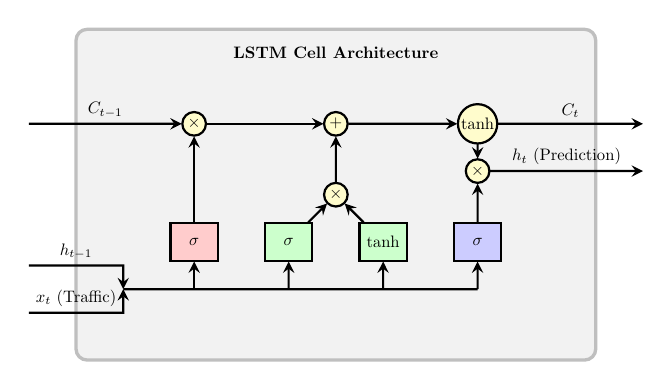
\begin{tikzpicture}[
        scale=0.6, transform shape,
        rect/.style={rectangle, draw, thick, minimum width=1cm, minimum height=0.8cm, fill=white},
        circ/.style={circle, draw, thick, minimum size=0.5cm, fill=yellow!20, inner sep=1pt},
        arrow/.style={->, >=stealth, thick},
        line/.style={-, thick}
    ]
        % Background
        \draw[rounded corners, fill=gray!10, draw=gray!50, very thick] (-2.5, -3.5) rectangle (8.5, 3.5);
        \node at (3, 3) {\textbf{LSTM Cell Architecture}};
        
        % Gates
        \node[rect, fill=red!20] (forget) at (0, -1) {$\sigma$};
        \node[rect, fill=green!20] (input_sig) at (2, -1) {$\sigma$};
        \node[rect, fill=green!20] (input_tanh) at (4, -1) {$\tanh$};
        \node[rect, fill=blue!20] (output) at (6, -1) {$\sigma$};
        
        % Ops
        \node[circ] (mul1) at (0, 1.5) {$\times$};
        \node[circ] (add1) at (3, 1.5) {$+$};
        \node[circ] (mul2) at (3, 0) {$\times$};
        \node[circ] (tanh2) at (6, 1.5) {$\tanh$};
        \node[circ] (mul3) at (6, 0.5) {$\times$};
        
        % Input Bus
        \coordinate (join) at (-1.5, -2);
        \draw[arrow] (-3.5, -2.5) -- node[above] {$x_t$ (Traffic)} (-1.5, -2.5) -- (join);
        \draw[arrow] (-3.5, -1.5) -- node[above] {$h_{t-1}$} (-1.5, -1.5) -- (join);
        \draw[line] (join) -- (6, -2);
        
        \draw[arrow] (0, -2) -- (forget.south);
        \draw[arrow] (2, -2) -- (input_sig.south);
        \draw[arrow] (4, -2) -- (input_tanh.south);
        \draw[arrow] (6, -2) -- (output.south);
        
        % Lines
        \draw[arrow] (-3.5, 1.5) -- node[above] {$C_{t-1}$} (mul1);
        \draw[arrow] (mul1) -- (add1);
        \draw[arrow] (add1) -- (tanh2);
        \draw[arrow] (tanh2) -- node[above] {$C_t$} (9.5, 1.5);
        
        \draw[arrow] (forget) -- (mul1);
        \draw[arrow] (input_sig) -- (mul2);
        \draw[arrow] (input_tanh) -- (mul2);
        \draw[arrow] (mul2) -- (add1);
        \draw[arrow] (tanh2) -- (mul3);
        \draw[arrow] (output) -- (mul3);
        \draw[arrow] (mul3) -- node[above] {$h_t$ (Prediction)} (9.5, 0.5);
    \end{tikzpicture}
    \end{center}
    \pause
    \begin{center}
        \alert{3 Cổng chính:} \textbf{Quên (Forget) - Đầu vào (Input) - Đầu ra (Output)} giúp LSTM lọc nhiễu cực tốt.
    \end{center}
\end{frame}

% SLIDE 6: Kiến trúc Hệ thống
\begin{frame}{Kiến trúc Tổng thể của Hệ thống}
    \begin{center}
    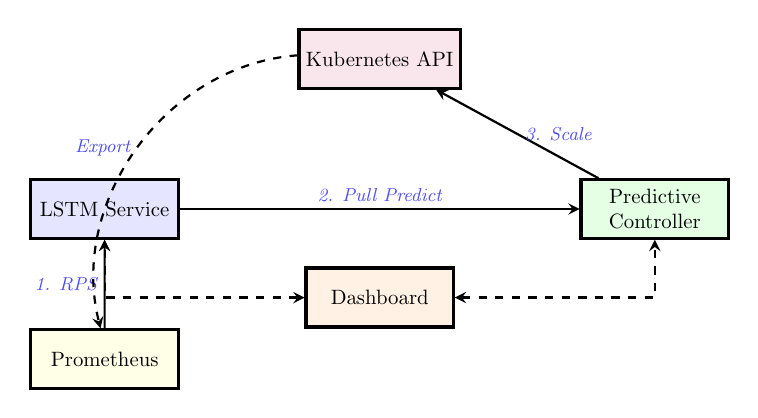
\begin{tikzpicture}[
        scale=0.75, transform shape,
        node distance=1.5cm and 2cm,
        box/.style={rectangle, draw=black, fill=white, very thick, minimum width=2.5cm, minimum height=1cm, align=center},
        arrow/.style={->, >=stealth, thick},
        label/.style={font=\small\itshape, text=blue!70}
    ]
        % Nodes
        \node[box, fill=purple!10] (k8s) {Kubernetes API};
        \node[box, fill=blue!10, below left=of k8s] (ml) {LSTM Service};
        \node[box, fill=green!10, below right=of k8s] (controller) {Predictive\\Controller};
        \node[box, fill=yellow!10, below=of ml] (prom) {Prometheus};
        \node[box, fill=orange!10, below=3cm of k8s] (dash) {Dashboard};
        
        % Arrows
        \draw[arrow] (prom) -- node[left, label] {1. RPS} (ml);
        \draw[arrow] (ml) -- node[above, label] {2. Pull Predict} (controller);
        \draw[arrow] (controller) -- node[right, label] {3. Scale} (k8s);
        \draw[arrow, dashed] (k8s) to[bend right=50] node[left, label] {Export} (prom);
        
        % Dash
        \draw[arrow, <->, dashed] (dash) -| (controller);
        \draw[arrow, <->, dashed] (dash) -| (ml);
    \end{tikzpicture}
    \end{center}
\end{frame}

% SLIDE 7: Smoothing Algorithm
\begin{frame}{Thuật toán Làm mịn (Chống Thrashing)}
    Bảo vệ Control Plane của Kubernetes khỏi các đợt "giật lag" khi model AI dự đoán biến động mạnh.
    \vspace{0.5cm}
    \begin{columns}
        \column{0.5\textwidth}
        \textbf{Quy tắc ràng buộc:}
        \begin{itemize}
            \item \textbf{Min-Max Bounds:} Không bé hơn 1, không lớn hơn 10.
            \item \textbf{Cửa sổ vận tốc:}
            \begin{itemize}
                \item Tăng nhanh: Tối đa +2 Pods / chu kỳ.
                \item Giảm chậm: Tối đa -1 Pod / chu kỳ.
            \end{itemize}
        \end{itemize}
        \column{0.5\textwidth}
        \begin{block}{Nguyên lý}
            "Mở rộng nhanh để chống nghẽn, Thu hẹp chậm để chống dư chấn (aftershocks)".
        \end{block}
    \end{columns}
\end{frame}

% SLIDE 8: Kịch bản Mô phỏng
\begin{frame}{Kịch bản Đỉnh tải 3 Pha (3-Phase Spike)}
    \begin{center}
    \begin{tikzpicture}[scale=0.9, transform shape]
        % Axes
        \draw[->, thick] (0,0) -- (10,0) node[right] {Thời gian};
        \draw[->, thick] (0,0) -- (0,5) node[above] {Số lượng Pods};
        
        % Phase lines (dashed vertical)
        \draw[dashed, gray] (3.3,0) -- (3.3,5);
        \draw[dashed, gray] (6.6,0) -- (6.6,5);
        
        % The graph
        \draw[thick, blue] (0,0.5) -- (3.3,4) -- (6.6,4) -- (10,0.5);
        
        % Phase Labels
        \node[text=red, font=\bfseries] at (1.65, 2.5) {1. Ramp Up};
        \node[text=green!60!black, font=\bfseries] at (4.95, 4.5) {2. Hold Peak};
        \node[text=purple, font=\bfseries] at (8.25, 2.5) {3. Ramp Down};
    \end{tikzpicture}
    \end{center}
\end{frame}

% SLIDE 9: Kết quả
\begin{frame}{Kết quả Thực nghiệm so sánh}
    \begin{table}
        \centering
        \begin{tabular}{lcc}
            \toprule
            \textbf{Chỉ số Đánh giá} & \textbf{Knative (Reactive)} & \textbf{Predictive (LSTM)} \\
            \midrule
            Khởi động lạnh (Cold Starts) & 100\% (Toàn bộ 9 Pods) & \textbf{\alert{0\% (Triệt tiêu)}} \pause \\
            Độ trễ trung bình đợt đầu & 3500 ms & \textbf{\alert{120 ms}} \pause \\
            Hiệu quả tài nguyên & 100\% & 92.5\% (Đánh đổi) \pause \\
            Thời gian đạt đỉnh 10 Pods & $\sim$45 giây & \textbf{20 giây} \\
            \bottomrule
        \end{tabular}
    \end{table}
    \pause
    \vspace{0.5cm}
    \begin{alertblock}{Kết luận nhanh}
        Đánh đổi $7.5\%$ lượng tài nguyên dư thừa tạm thời để đổi lấy tốc độ phản hồi \textbf{nhanh hơn gấp 29 lần}!
    \end{alertblock}
\end{frame}

% SLIDE 10: Tổng kết
\begin{frame}{Tổng kết \& Hướng phát triển}
    \textbf{Đóng góp của đề tài:}
    \begin{itemize}
        \item Khắc phục hoàn toàn bài toán Cold-start trong Serverless (Knative).
        \item Tích hợp thành công AI (LSTM) vào hệ sinh thái DevOps/Kubernetes.
        \item Xây dựng Controller giám sát độc lập, an toàn (Smoothing).
    \end{itemize}
    \vspace{0.5cm}
    \pause
    \textbf{Hướng phát triển tương lai:}
    \begin{itemize}
        \item Huấn luyện mô hình Transformer thay vì LSTM để tăng tốc.
        \item Thu thập dữ liệu thực tế (Real-world datasets) từ các sàn E-commerce.
    \end{itemize}
\end{frame}

\end{document}
